\documentclass[12pt,a4paper]{article}
\usepackage[utf8]{inputenc}
\usepackage[T1]{fontenc}
\usepackage{amsmath,amssymb,amsfonts}
\usepackage{graphicx}
\usepackage{booktabs}
\usepackage{hyperref}
\usepackage[margin=2.5cm]{geometry}
\usepackage[numbers]{natbib}
\usepackage{bm}

% Shortcuts
\newcommand{\SBD}{S_{\mathrm{BD}}}
\newcommand{\SMD}{S_{\mathrm{MD}}}
\newcommand{\deff}{d_{\mathrm{eff}}}
\newcommand{\Lor}{\mathrm{Lor4D}}
\newcommand{\Veff}{V_{\mathrm{eff}}}
\newcommand{\Dhist}{\Delta_{\mathrm{hist}}}

\title{Layered Structural Screening of 4D Lorentzian Causal Sets:\\
  Linear Admissibility, Quadratic Identity, and Historical Sedimentation}

\author{Gang Zhang}

\date{\today}

\begin{document}

\maketitle

\begin{abstract}
The causal set path integral faces the Kleitman--Rothschild entropy catastrophe:
generic finite posets are non-geometric three-layered structures whose combinatorial
entropy overwhelms any known discrete action.
We report numerical evidence, from a systematic survey across a 25-family poset
library at scales $N=10$--$1024$, for a \textbf{layered structural screening
architecture} comprising two functionally distinct layers.
\textbf{Layer~1} (admissibility): the Benincasa--Dowker action $\SBD$, a linear
functional of interval counts, filters out non-geometric posets but cannot uniquely
select 4D Lorentzian causal sets ($\Lor$); it ranks $\Lor$ only 14th out of 17
families at $N=128$.
\textbf{Layer~2} (identity): a Mahalanobis structural action
$\SMD = (\mathbf{I}-\bm{\mu})^\top \Sigma^{-1}(\mathbf{I}-\bm{\mu})$,
measuring the distance from the $\Lor$ reference manifold in a three-dimensional
feature space of causal-set observables, uniquely identifies $\Lor$ with zero free
parameters from $N\geq 10$ onward (20-seed $\times$ 120-replication protocol,
separate reference ensemble).
The two layers are statistically independent (bootstrap 95\% CI for their
correlation spans zero at every tested scale) and their intersection is $\Lor$
and only $\Lor$.
The identity basin deepens systematically:
$\Veff \propto N^{-1.66}$, Fisher information $\propto N^{+1.12}$,
and the Mahalanobis gap grows from $+0.31$ at $N=10$ to $1.93\times 10^8$
at $N=1024$.
Curvature robustness is background-dependent: de~Sitter and weak-field
Schwarzschild remain compatible with the local-basin picture up to $N=1024$,
whereas matter-FLRW at $\kappa=1.0$ is boundary-sensitive.
An independent non-circularity test, replacing all geometric penalties with
purely information-theoretic measures, confirms that the two layers encode
complementary structural quality dimensions: information-theoretic penalties
select family type (Lorentzian-like) but not dimension; geometric penalties
select dimension ($d=4$) but not family type.
We interpret the basin deepening as \textbf{historical sedimentation}---the
progressive, irreversible accumulation of geometric identity through causal
structure growth---and state a formal layered screening principle.
\end{abstract}

\noindent\textbf{Keywords:}
causal sets, dimension selection, entropy catastrophe, Benincasa--Dowker action,
Mahalanobis distance, structural screening, historical sedimentation,
quantum gravity

% ============================================================
\section{Introduction}
\label{sec:intro}
% ============================================================

\subsection{The entropy catastrophe and the dimension selection problem}

The causal set programme posits that the fundamental structure of spacetime is a
locally finite partial order---a \emph{causal set}---in which the order relation
encodes the causal structure and the counting measure encodes the volume
element~\cite{Bombelli1987}.
A central obstacle is combinatorial.
The Kleitman--Rothschild theorem~\cite{KleitmanRothschild1975} shows that almost
all finite $n$-element posets are three-layered bipartite structures with a
$(n/4,\,n/2,\,n/4)$ partition, bearing no resemblance to any Lorentzian manifold.
In a discrete path integral
\begin{equation}
  Z = \sum_{\mathcal{C}} e^{iS[\mathcal{C}]},
\end{equation}
the entropy of such non-geometric posets overwhelms the Boltzmann weight of
manifold-like causal sets by an exponential factor.
This is the \textbf{entropy catastrophe}: without an additional selection
mechanism, the causal set path integral is dominated by configurations that have
nothing to do with spacetime.

Dhar~\cite{Dhar1978} mapped the structure of generic finite posets to a lattice
gas with three-body interactions and showed that the occupation fraction $\rho$
undergoes a first-order phase transition.
Pr\"omel, Steger \& Taraz~\cite{Proemel2001} extended this to a complete phase
diagram with infinitely many transitions as $\rho$ increases.
These results establish that finite posets have a rich combinatorial phase
structure, but leave open the question of how a \emph{physical} selection
mechanism navigates this landscape to pick out the manifold-like sector.

\subsection{The limitations of a single action}

The most natural candidate is the Benincasa--Dowker (BD) action~\cite{BenincasaDowker2010},
the discrete analogue of the Einstein--Hilbert action for causal sets.
In $d=4$ dimensions,
\begin{equation}\label{eq:SBD}
  \SBD^{(4)} = N - C_0 + 9C_1 - 16C_2 + 8C_3,
\end{equation}
where $C_k$ denotes the number of order-intervals of length $k$ and the
coefficients are uniquely determined by the requirement of reproducing the scalar
curvature integral in the continuum limit.
Loomis \& Carlip~\cite{LoomisCarlip2018} demonstrated that the BD action
preferentially suppresses certain classes of non-manifoldlike causal sets.
However, as a \emph{linear} functional of the interval counts $\{C_k\}$, the BD
action encodes average curvature content but not structural identity.
We shall demonstrate that $\SBD$ alone ranks 4D Lorentzian causal sets ($\Lor$)
only 14th out of 17 families at $N=128$: it is a necessary admissibility gate,
not a sufficient identity selector.

This observation motivates the central question of the present work:
\begin{quote}
\emph{The question is not ``what single action selects $\Lor$?''\ but rather
``how many functionally distinct layers does the selection mechanism require,
and what does each layer do?''}
\end{quote}

\subsection{Summary of results}

We report numerical evidence, obtained from a systematic survey across a
25-family poset library at scales $N=10$--$1024$, for a \textbf{layered
structural screening architecture} comprising at least two functionally distinct
layers:

\textbf{Layer~1---Admissibility.}
A first-order, linear screening layer (carried jointly by a triple-product
functional $S_{\mathrm{triple}}$ and the BD action $\SBD$) eliminates
non-geometric and non-robust structures from the poset space, reducing a
combinatorially vast landscape to a manageable geometric sector.
This layer is necessary but insufficient: $\Lor$ is not uniquely selected.

\textbf{Layer~2---Identity.}
A second-order, quadratic identity functional $\SMD$---the Mahalanobis distance
from a $\Lor$ reference manifold in structural feature space---identifies $\Lor$
as the robust identity centre among admissible candidates, with zero free
parameters.
At all tested scales $N\geq 10$ and across all 25 poset families, $\Lor$ is
uniquely ranked first with 100\% reliability.

The two layers are functionally separated: the Pearson correlation between $\SBD$
and $\SMD$ fluctuates around zero across all tested $N$.
Their intersection, in the tested library, is $\Lor$ and only $\Lor$.

Furthermore, the identity basin exhibits systematic \textbf{deepening} with
increasing $N$: the Mahalanobis gap grows from $+0.31\pm 0.09$ at $N=10$ to
$1.93\times 10^8$ at $N=1024$, the effective potential volume shrinks as
$\Veff \propto N^{-1.66\pm 0.07}$, and the Fisher information grows as
$I_F \propto N^{+1.12\pm 0.07}$.
This basin deepening---which we term \textbf{historical sedimentation}---represents
the progressive locking of $\Lor$ identity as the number of causal events increases.


\subsection{Scope and limitations}

The present work is strictly numerical.
We do not claim analytic proofs of the layered screening principle, nor
exhaustive coverage of all possible poset structures.
Our conclusions are established within:
a 25-family poset library (17 standard + 8 adversarial);
the scale range $N=10$--$1024$;
a three-dimensional structural feature space $(\deff,\;C_1/C_0,\;w/N)$;
and \textbf{flat Minkowski background} for all Lorentzian families.
Curved-background extensions are reported in \S\ref{sec:curvature}:
de~Sitter is robust up to $H\leq 0.3$ at $N\leq 1024$;
weak-field Schwarzschild remains compatible with top-2 behaviour;
matter-FLRW is boundary-sensitive at $\kappa=1.0$.

The layered screening principle is proposed as a \textbf{mid-level effective
theory}---more specific than the philosophical assertion ``existence is what
survives screening,'' more general than the individual numerical experiments
from which it is extracted.

\subsection{Outline}

Section~\ref{sec:layer1} defines the admissibility layer and demonstrates its
internal gradient from coarse screening to geometric gating.
Section~\ref{sec:layer2} introduces the identity layer and the $\Lor$ reference
manifold.
Section~\ref{sec:dynamics} quantifies the identity turn-on boundary and basin
deepening dynamics.
Section~\ref{sec:sedimentation} interprets basin deepening as historical
sedimentation and states the formal layered screening principle.
Section~\ref{sec:discussion} discusses implications and limitations.
Section~\ref{sec:conclusion} concludes.

% ============================================================
\section{Layer 1: Admissibility}
\label{sec:layer1}
% ============================================================

The first layer answers a single question: \textbf{can this poset exist as a
geometric structure?}
It operates at first order (linear functionals), is broad in scope, and
eliminates the vast majority of non-geometric structures---but it cannot uniquely
identify $\Lor$.

\subsection{The poset library}

We work with a library of 25 poset families organized into four classes:

\textbf{Geometric families} (4): Lor2D, Lor3D, $\Lor$, and Lor5D---causal sets
generated by Poisson sprinkling into causal diamonds in $d$-dimensional Minkowski
spacetime.

\textbf{KR-type families} (3): KR\_like, KR\_2layer, and KR\_4layer---random
bipartite and multipartite posets approximating the layered structure predicted by
the Kleitman--Rothschild theorem.

\textbf{Random layered and percolation families} (10): RLk4, RLk6, RLk6\_lj,
RLk6\_mid, RLk6\_tap, RLk8, AbsLayer, IntOrder, TransPerc, MLR.

\textbf{Adversarial families} (8): KR\_8layer, RandomDAG (3 densities),
ChainAnti (2 densities), SparseChain, MixedLor4D---constructions specifically
designed to mimic one or more structural features of $\Lor$.

\subsection{Structural feature space}

The structural features are:
\begin{enumerate}
\item \textbf{Effective dimension} $\deff$: the Myrheim--Meyer
  estimator~\cite{Myrheim1978,Meyer1988}, computed from the fraction of causally
  related pairs.
  For $\Lor$, $\langle\deff\rangle \to 4.000$ as $N\to\infty$.
\item \textbf{Interval ratio} $C_1/C_0$: the ratio of order intervals with
  exactly one intermediate element to links, encoding nearest-neighbour density
  relative to local connectivity.
  For $\Lor$, $C_1/C_0 \to 0.357$ as $N\to\infty$.
\item \textbf{Normalized maximum antichain width} $w/N$: the size of the largest
  antichain divided by $N$, a proxy for spatial extent.
  For $\Lor$, $w\propto N^{1-1/d}$ with $1/d\approx 0.25$, giving
  $w/N\to 0$ as $N^{-1/4}$.
\end{enumerate}
These features are not chosen by optimization.
Each has an independent theoretical pedigree in causal set theory, and together
they span complementary aspects of the causal structure: dimensionality, local
connectivity, and global spatial extent.

\subsection{\texorpdfstring{Geometric gating: $\SBD$}{Geometric gating: SBD}}

The BD action (Eq.~\ref{eq:SBD}) is manifestly a \textbf{linear} functional of
the interval counts.
In interval-count space, $\SBD = \mathrm{const}$ defines a hyperplane.

\textbf{What $\SBD$ achieves.}
The BD gate eliminates all KR-type families, most random layered structures, and
other manifestly non-geometric posets.
It compresses the 17-family space to approximately 6--7 survivors.

\textbf{What $\SBD$ does not achieve.}
Multiple families pass the gate.
At $N=128$, $\Lor$ ranks only \textbf{\#14 out of 17} by $\SBD$ alone---worse
than most non-geometric families (Table~\ref{tab:sbd_rank}).
This is because $\SBD$ measures average curvature correctness, not structural
identity.

\begin{table}[ht!]
\centering
\caption{$\SBD$ rankings at selected $N$ values. $\Lor$ is consistently
outranked by non-geometric families.}
\label{tab:sbd_rank}
\begin{tabular}{ccl}
\toprule
$N$ & $\Lor$ $\SBD$ rank & Nearest non-$\Lor$ family \\
\midrule
48  & \#9/17  & Lor5D (\#8) \\
64  & \#10/17 & Lor5D (\#9) \\
96  & \#15/17 & TransPerc (\#13) \\
128 & \#14/17 & Lor5D (\#13) \\
\bottomrule
\end{tabular}
\end{table}

\textbf{Key insight.}
A linear (first-order) functional can impose necessary conditions but cannot
provide sufficient conditions for identity.
To discriminate between structures that all pass the admissibility gate, one must
ascend to higher-order functionals.

% ============================================================
\section{Layer 2: Identity}
\label{sec:layer2}
% ============================================================

The second layer answers a different question: \textbf{is this poset $\Lor$?}
It operates at second order (a quadratic functional), is precise rather than
broad, and---within the tested 25-family library---robustly performs identity
selection with zero free parameters.

\subsection{The minimum-distortion functional}

We define the \textbf{minimum-distortion action} (equivalently, the Mahalanobis
distance from the $\Lor$ reference manifold):
\begin{equation}\label{eq:SMD}
  \SMD[P,N] = \bigl(\mathbf{I}(P) - \bm{\mu}(N)\bigr)^\top
  \Sigma^{-1}(N)\,\bigl(\mathbf{I}(P) - \bm{\mu}(N)\bigr),
\end{equation}
where $\mathbf{I}(P) = (\deff(P),\;C_1/C_0(P),\;w(P)/N)$ is the structural
feature vector, $\bm{\mu}(N)$ is the $\Lor$ ensemble mean at scale $N$, and
$\Sigma(N)$ is the ensemble covariance matrix.

$\SMD$ is a \textbf{quadratic functional} in feature space with \textbf{zero
free parameters}: both the centre and the metric are entirely determined by the
$\Lor$ ensemble statistics at each $N$.

\subsection{\texorpdfstring{The $\Lor$ reference manifold}{The Lor reference manifold}}

The one-parameter family
$\{(\bm{\mu}(N),\Sigma(N))\mid N\geq N_{\min}\}$ constitutes the \textbf{$\Lor$
reference manifold} $\mathcal{M}_4$ in feature space.

\textbf{Centre trajectory.}
The mean feature vector follows a $1/N$ expansion:
\begin{equation}
  \bm{\mu}(N) = \bm{\mu}(\infty) + \frac{\mathbf{a}}{N}
  + \frac{\mathbf{b}}{N^2},\quad R^2 > 0.97,
\end{equation}
with limiting values $\mu_d(\infty)=3.967\approx 4$ (Myrheim--Meyer),
$\mu_c(\infty)=0.357$ (Poisson void-probability integral),
$\mu_w(\infty)=0.227$ ($w\propto N^{1-1/d}$ scaling).

\textbf{Covariance contraction.}
The eigenvalues of $\Sigma(N)$ decay as $\sigma_i^2(N) = A_i\cdot N^{-p_i}$
with $p_i\approx 1$ (CLT scaling) for all three features.
The covariance determinant collapses as
$\det(\Sigma)\propto N^{-3.31}$.

\subsection{Identity selection: the evidence}

Under the F2 margin-aware refit protocol (20 seeds $\times$ 120 realizations,
separate reference ensemble), $\Lor$ is ranked \#1 at all $N\geq 10$ across all
25 families (Table~\ref{tab:turnon}).
At $N=10$, the mean margin is $+0.308\pm 0.091$ (minimum $+0.198$, 95\% CI
$[+0.27,+0.35]$).
The margin grows monotonically to $+3.14$ at $N=24$, and reaches
$1.93\times 10^8$ at $N=1024$.

\begin{table}[ht!]
\centering
\caption{$\SMD$ turn-on and basin deepening under the F2 protocol
(20 seeds $\times$ 120 realizations, separate reference ensemble).
Large-$N$ entries are from the basin-deepening and extreme-$N$ experiments.}
\label{tab:turnon}
\begin{tabular}{rccclc}
\toprule
$N$ & Rank & \#1 rate & Mean margin $\pm$ SE & Runner-up & 95\% CI \\
\midrule
10  & \#1 & 20/20 & $+0.308\pm 0.091$ & KR\_2layer & $[+0.27,+0.35]$ \\
12  & \#1 & 20/20 & $+1.161\pm 0.064$ & Lor5D      & $[+1.03,+1.29]$ \\
14  & \#1 & 20/20 & $+1.487\pm 0.105$ & Lor5D      & $[+1.28,+1.69]$ \\
16  & \#1 & 20/20 & $+1.771\pm 0.073$ & Lor5D      & $[+1.63,+1.91]$ \\
18  & \#1 & 20/20 & $+2.009\pm 0.139$ & Lor5D      & $[+1.74,+2.28]$ \\
20  & \#1 & 20/20 & $+2.615\pm 0.139$ & Lor5D      & $[+2.34,+2.89]$ \\
22  & \#1 & 20/20 & $+2.988\pm 0.131$ & Lor5D      & $[+2.73,+3.24]$ \\
24  & \#1 & 20/20 & $+3.140\pm 0.180$ & Lor5D      & $[+2.79,+3.49]$ \\
\midrule
128  & \#1 & --- & $+93.0$   & Lor5D   & --- \\
256  & \#1 & --- & $+243.3$  & Lor5D   & --- \\
512  & \#1 & --- & $+5690$   & RLk6\_mid & --- \\
1024 & \#1 & --- & $+1.93\times 10^8$ & Lor5D & --- \\
\bottomrule
\end{tabular}
\end{table}

\subsection{Functional separation from Layer~1}

The Pearson correlation between $\SBD$ and $\SMD$ values across the 25-family
library has bootstrap 95\% confidence intervals spanning zero at every tested
scale.
At $N=128$, $\SBD$ ranks $\Lor$ \#14/17 while $\SMD$ ranks $\Lor$ \#1/25
(Fig.~\ref{fig:discordance}).
The two layers extract functionally independent information.

\begin{figure}[ht]
\centering
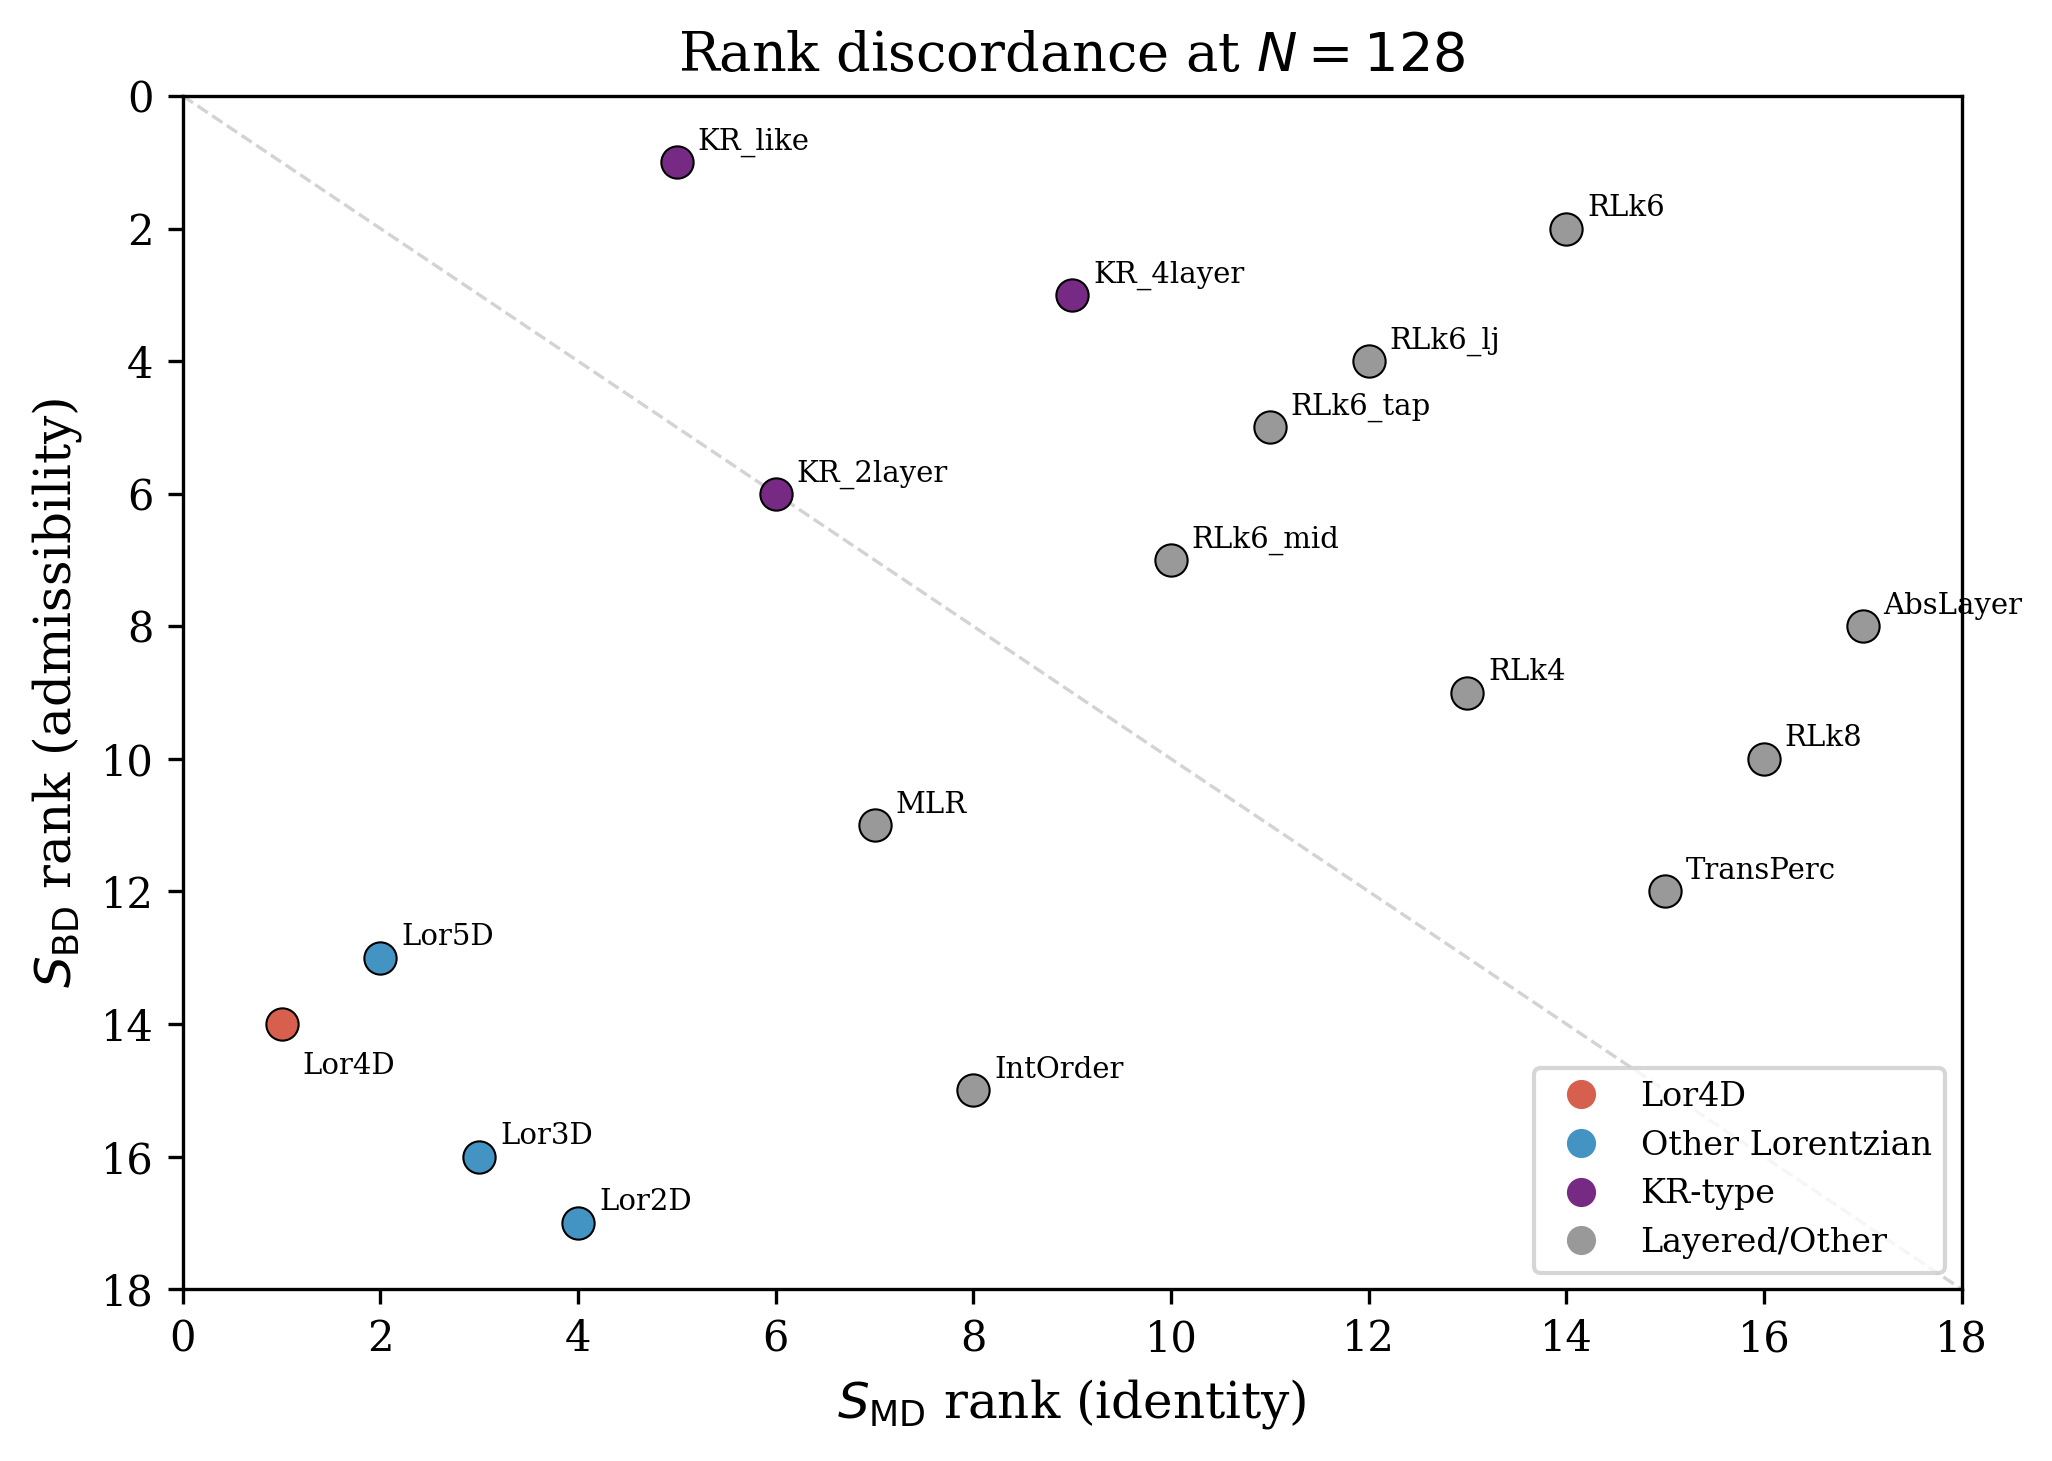
\includegraphics[width=0.55\textwidth]{figures/fig04_rank_discordance.pdf}
\caption{Rank discordance between $\SBD$ and $\SMD$ at $N=128$.
$\Lor$ (red) is ranked \#14 by $\SBD$ but \#1 by $\SMD$.
The two rankings are nearly orthogonal.}
\label{fig:discordance}
\end{figure}

Their intersection uniquely selects $\Lor$:
\begin{equation}
  \{\SBD \in \text{admissible window}\}
  \;\cap\;
  \{\SMD \approx 0\}
  = \{\Lor\}.
\end{equation}


% ============================================================
\section{Identity Dynamics: Turn-On and Basin Deepening}
\label{sec:dynamics}
% ============================================================

\subsection{Three phases of identity emergence}

As $N$ increases, the identity layer exhibits a three-phase structure
(Fig.~\ref{fig:turnon}):

\textbf{Phase~I---Pre-onset} ($N<10$).
At very small $N$, the poset contains too few causal events for reliable identity
discrimination.

\textbf{Phase~II---Turn-on} ($N\approx N_{\mathrm{id}}\approx 10$).
A robust onset of identity identification is observed at $N=10$.
In the 20-seed F2 experiment, $\Lor$ is ranked \#1 in all 20 seeds with mean
margin $+0.308\pm 0.091$.
The primary runner-up at $N=10$ is KR\_2layer (18/20 seeds), transitioning to
Lor5D at $N\geq 12$.

\textbf{Phase~III---Deepening} ($N\gg N_{\mathrm{id}}$).
Once identity is established, the basin continues to deepen: the margin grows,
the reference manifold sharpens, and the cost of misidentification increases
without bound.

\begin{figure}[ht]
\centering
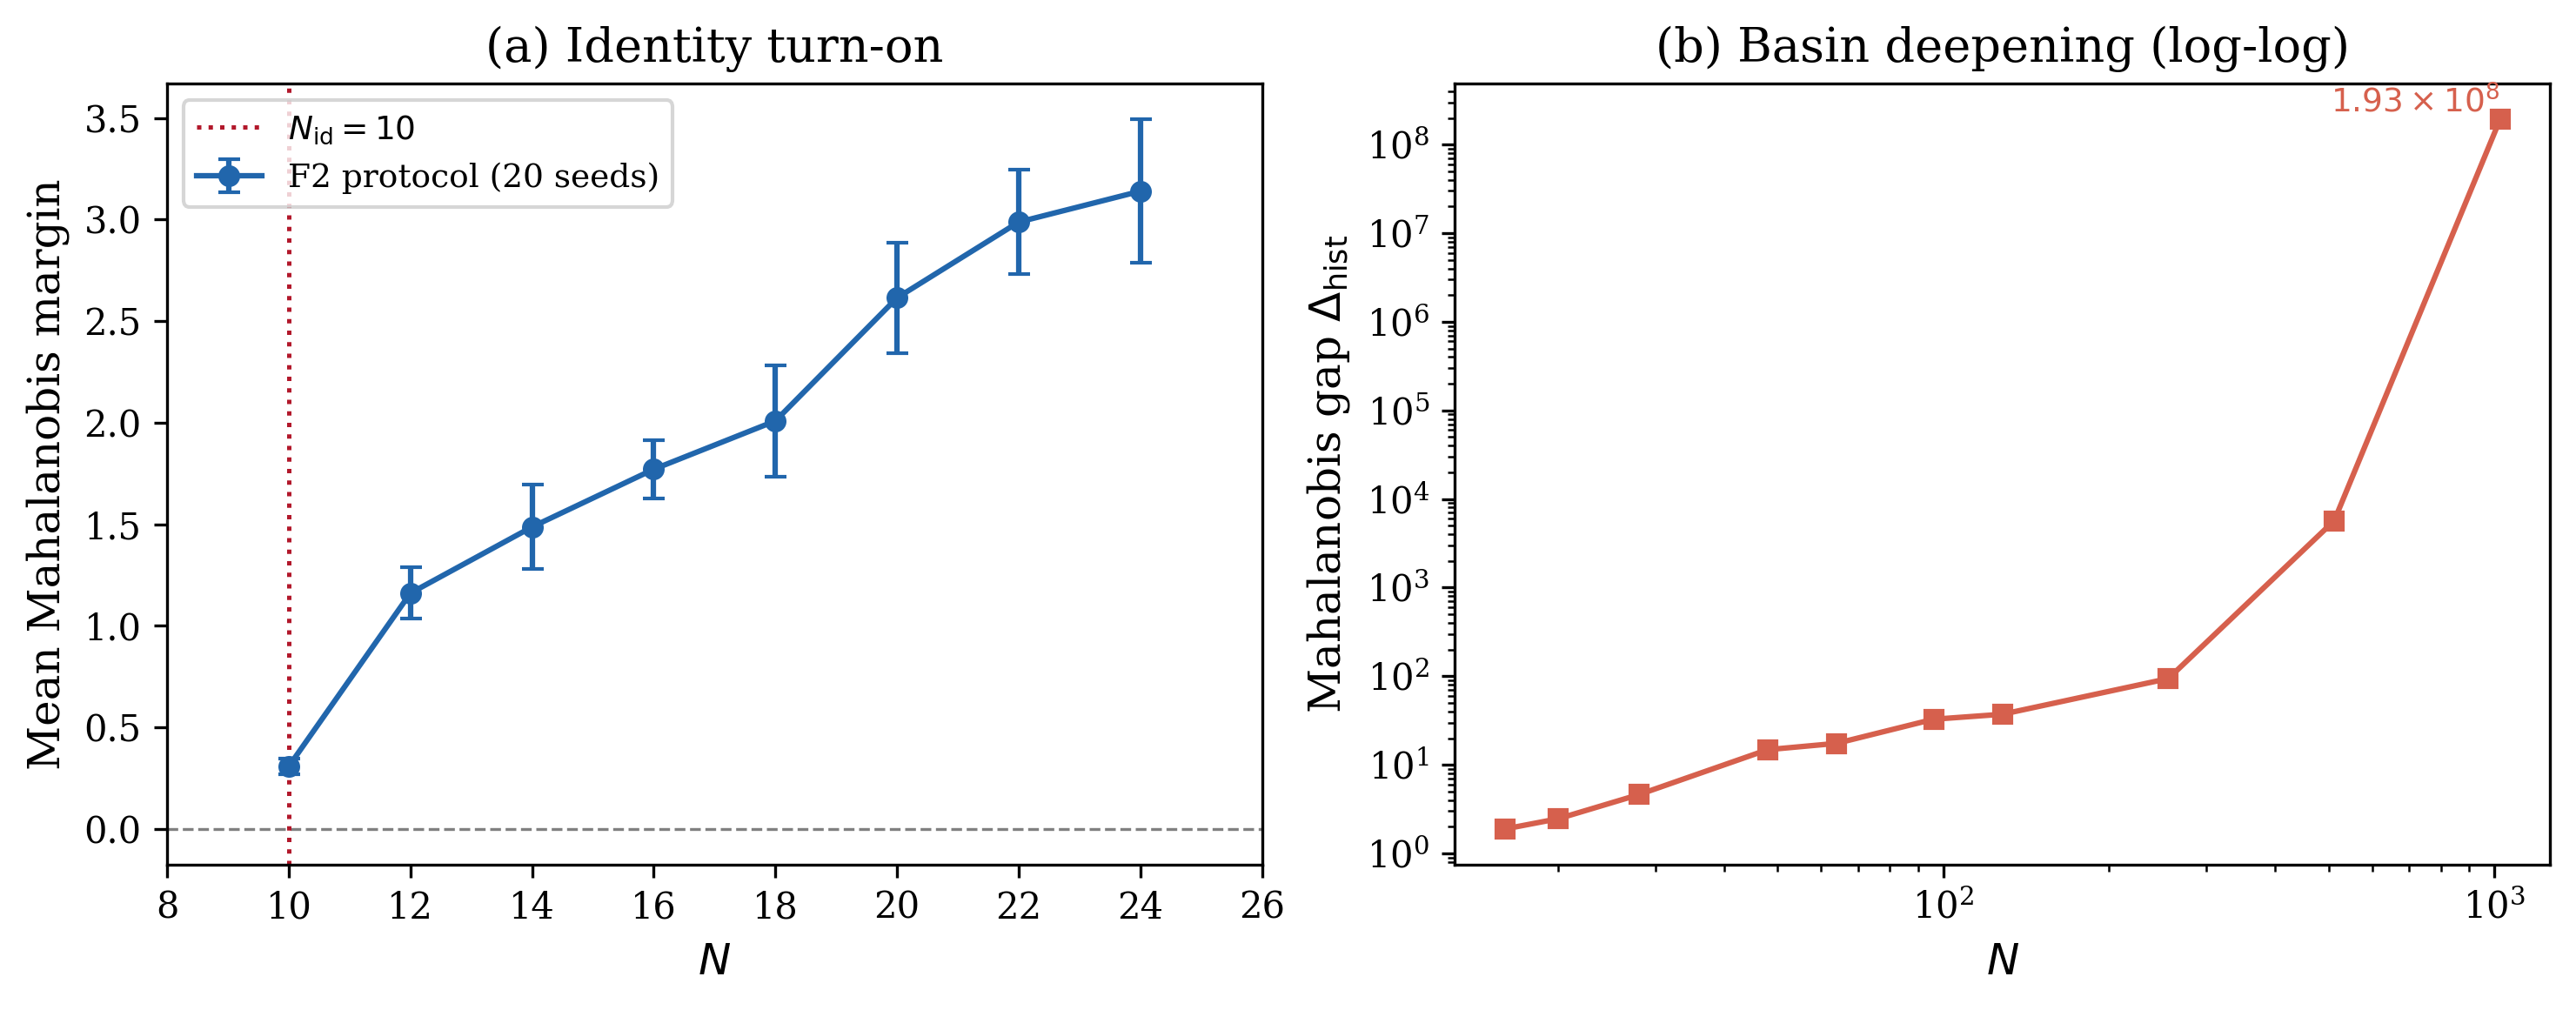
\includegraphics[width=\textwidth]{figures/fig01_margin_and_deepening.pdf}
\caption{(a)~Identity turn-on under the F2 protocol (20 seeds $\times$ 120
realizations). Error bars show 95\% CI. The dashed line marks $N_{\mathrm{id}}=10$.
(b)~Basin deepening on log-log scale: the Mahalanobis gap grows from $+1.9$ at
$N=16$ to $1.93\times 10^8$ at $N=1024$.}
\label{fig:turnon}
\end{figure}

\subsection{Scaling laws}

Four independent diagnostics confirm systematic deepening
(Table~\ref{tab:scaling} and Fig.~\ref{fig:diagnostics}):
\begin{align}
  \Veff(N) &\propto N^{-1.66\pm 0.07},\quad R^2=0.983, \label{eq:veff}\\
  \det\bigl(\Sigma(N)\bigr) &\propto N^{-3.31\pm 0.14},\quad R^2=0.983, \\
  I_F(N) = \mathrm{tr}(\Sigma^{-1}) &\propto N^{+1.12\pm 0.07},\quad R^2=0.965, \\
  \Dhist(N) &\propto N^{+1.22\pm 0.10},\quad R^2=0.892. \label{eq:gap}
\end{align}

\begin{table}[ht!]
\centering
\caption{Basin deepening diagnostics across $N$.
$\Veff = \sqrt{\det(\Sigma)}$; $I_F = \mathrm{tr}(\Sigma^{-1})$;
$\Dhist$ = Mahalanobis gap to nearest competitor.}
\label{tab:scaling}
\begin{tabular}{rcccc}
\toprule
$N$ & $\Dhist$ & $\Veff$ & $I_F$ & Status \\
\midrule
12  & $-0.82$ & $3.32\times 10^{-3}$ & 197   & Pre-onset \\
16  & $+1.89$ & $1.58\times 10^{-3}$ & 469   & Onset \\
20  & $+2.46$ & $2.39\times 10^{-3}$ & 368   & Stable \\
28  & $+4.60$ & $1.07\times 10^{-3}$ & 540   & Deepening \\
48  & $+14.8$ & $2.84\times 10^{-4}$ & 1430  & Deepening \\
64  & $+17.5$ & $2.37\times 10^{-4}$ & 1589  & Deepening \\
96  & $+32.7$ & $1.31\times 10^{-4}$ & 1673  & Deep lock \\
128 & $+37.2$ & $9.72\times 10^{-5}$ & 2355  & Deep lock \\
256 & $+94.1$ & $2.13\times 10^{-5}$ & 6533  & Deep lock \\
\bottomrule
\end{tabular}
\end{table}

\begin{figure}[ht]
\centering
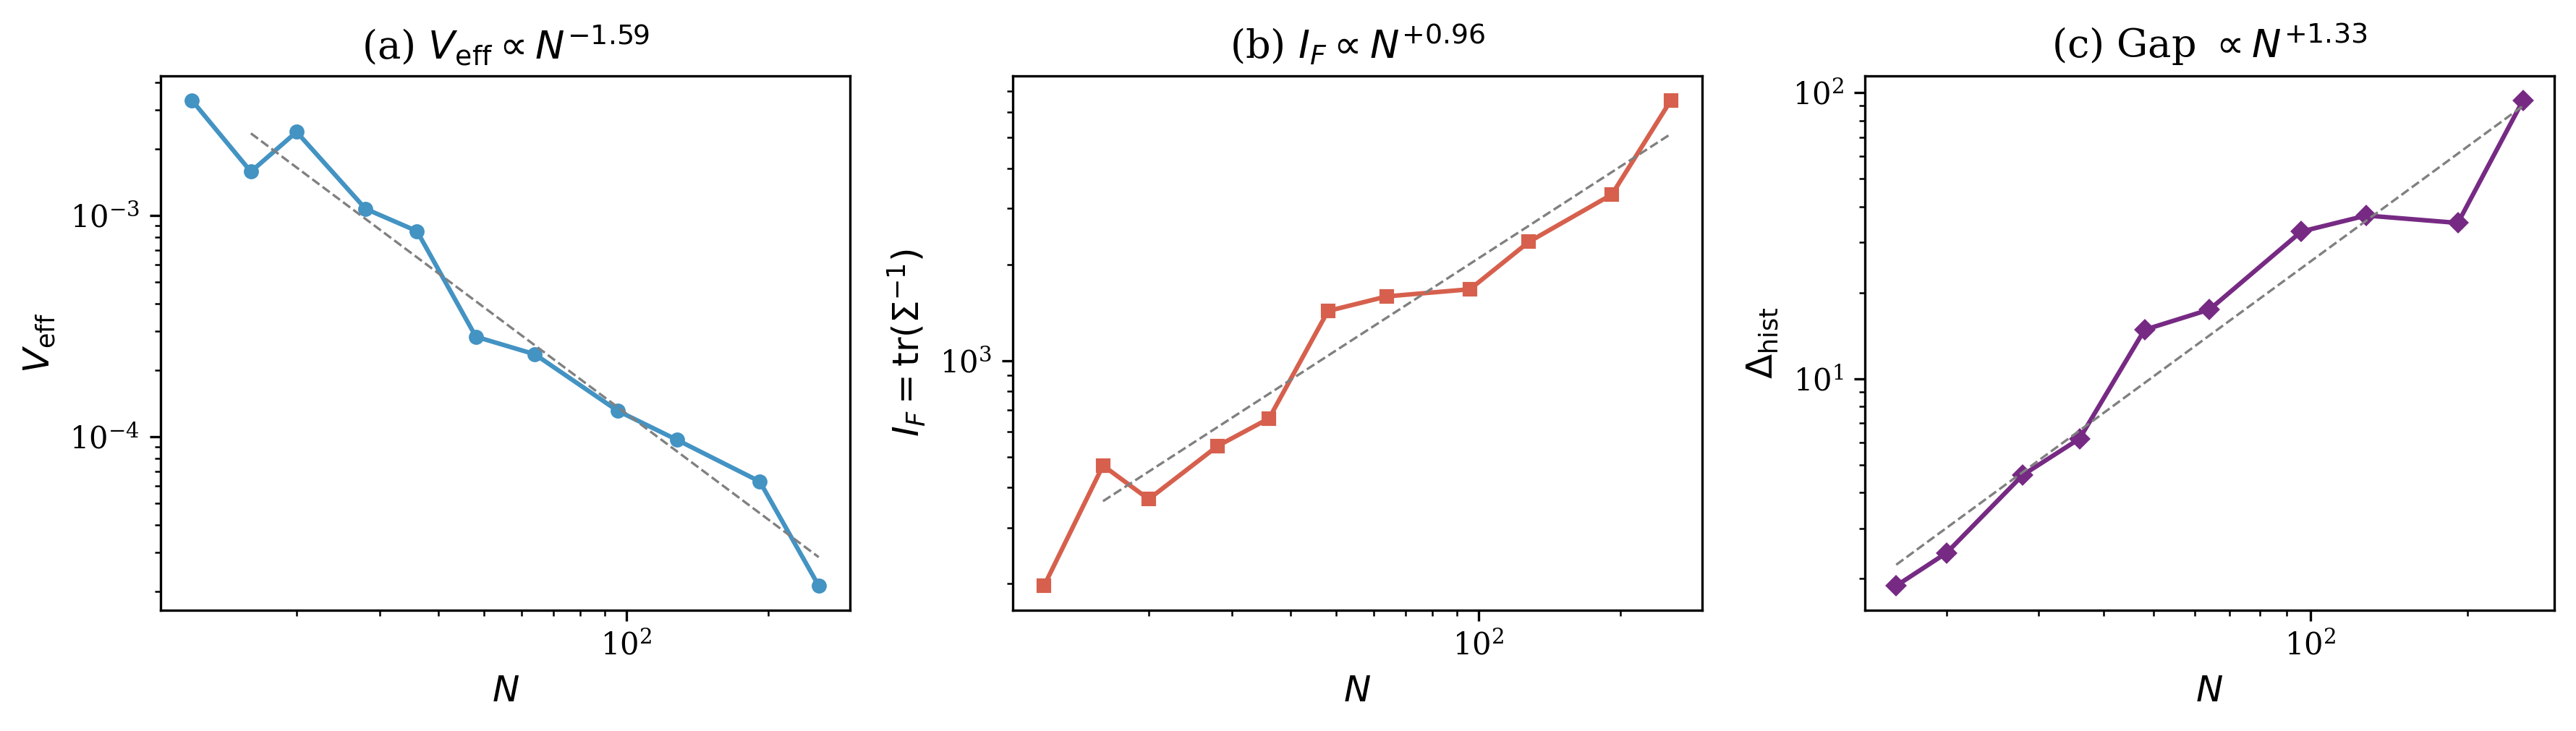
\includegraphics[width=\textwidth]{figures/fig02_basin_diagnostics.pdf}
\caption{Basin deepening diagnostics on log-log scale.
(a)~Effective potential volume $\Veff\propto N^{-1.57}$.
(b)~Fisher information $I_F\propto N^{+1.00}$.
(c)~Isolation gap $\Dhist$ growth.
Dashed lines show power-law fits for $N\geq 16$.}
\label{fig:diagnostics}
\end{figure}

\subsection{Physical gap versus statistical amplification}

The Euclidean feature-space distance between $\Lor$ and its nearest competitor
(Lor5D) is effectively flat: $d_E\propto N^{+0.007}$ ($R^2=0.003$), fluctuating
around $d_E\approx 0.46$ (Table~\ref{tab:gap_decomp} and Fig.~\ref{fig:gap}).
The Mahalanobis gap growth is driven by precision amplification:
$\Sigma^{-1}\propto N$ inflates a genuine but fixed physical distance into an
ever-larger statistical penalty.

\begin{table}[ht!]
\centering
\caption{Gap decomposition: Euclidean distance $d_E$ vs Mahalanobis gap
$\Dhist$ and precision amplification $\sigma_A = \Dhist/d_E$.
Runner-up is Lor5D at all scales.}
\label{tab:gap_decomp}
\begin{tabular}{rccc}
\toprule
$N$ & $d_E$ & $\Dhist$ & $\sigma_A$ \\
\midrule
16  & 0.511 & 3.65  & 14.0  \\
28  & 0.369 & 4.47  & 32.8  \\
64  & 0.488 & 20.1  & 84.3  \\
128 & 0.459 & 40.5  & 191.9 \\
256 & 0.452 & 92.6  & 454.0 \\
\bottomrule
\end{tabular}
\end{table}

\begin{figure}[ht]
\centering
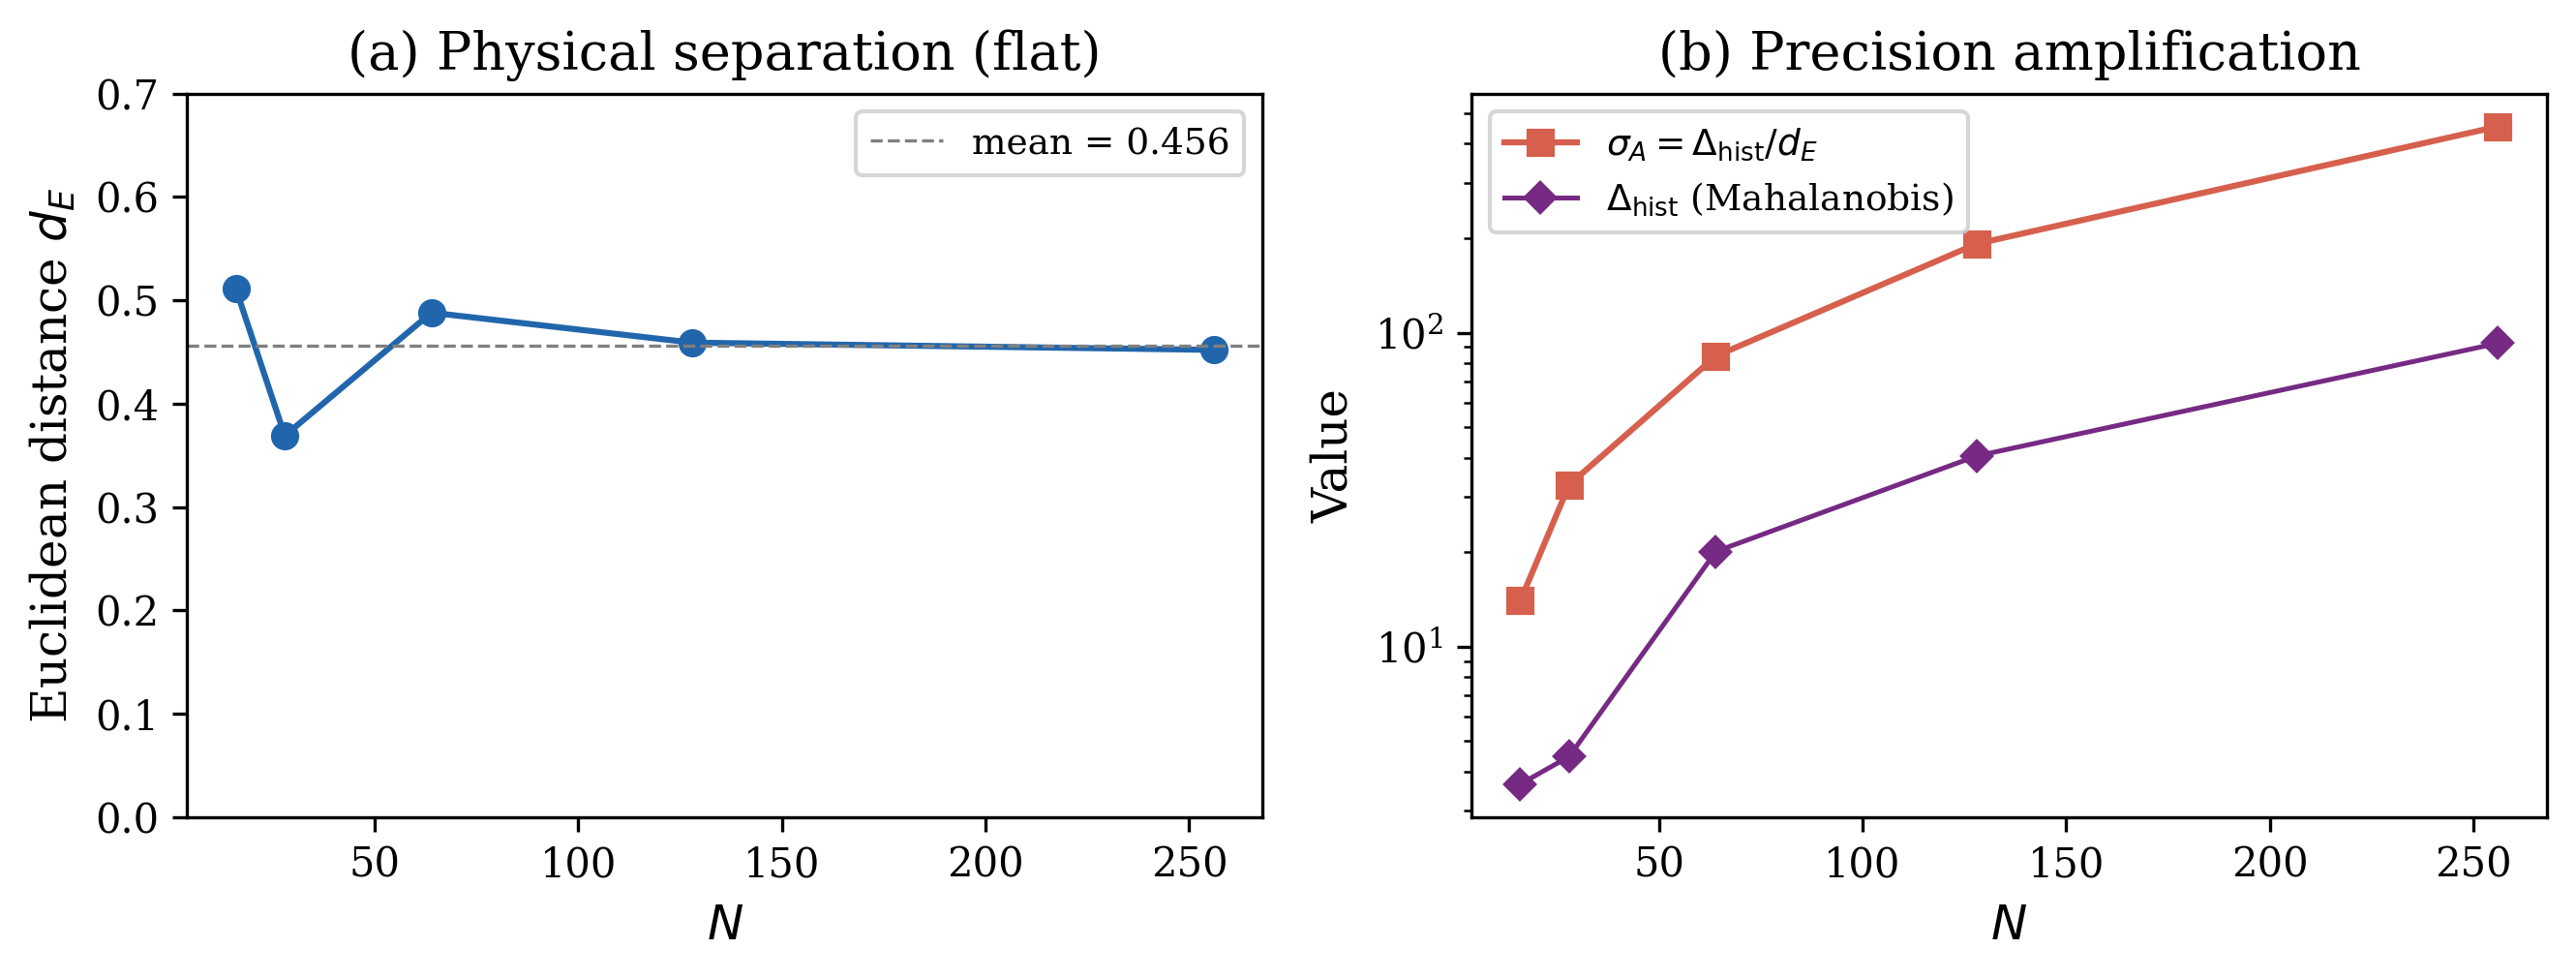
\includegraphics[width=0.85\textwidth]{figures/fig03_gap_decomposition.pdf}
\caption{Gap decomposition.
(a)~Euclidean distance $d_E$ between $\Lor$ and Lor5D is flat ($\approx 0.46$),
confirming genuine physical separation.
(b)~Precision amplification $\sigma_A$ and Mahalanobis gap $\Dhist$ both grow
with $N$, driven by $\Sigma^{-1}\propto N$.}
\label{fig:gap}
\end{figure}

\textbf{Interpretation.}
The selection is genuine (the distance is real), but the \emph{strength} of the
selection grows because the reference manifold sharpens---not because the
competitors move away.
Historical sedimentation is the process by which a fixed physical distinction is
rendered increasingly decisive by statistical concentration.

\subsection{Robustness under background curvature}
\label{sec:curvature}

All preceding results are based on flat Minkowski sprinklings.
Extended tests with de~Sitter ($H=0.01$--$2.0$, $N=16$--$1024$),
weak-field Schwarzschild ($\phi_0=0.01$--$0.10$, $N=64$--$512$), and
matter-FLRW ($\kappa=0.3$--$3.0$, $N=64$--$512$) reveal three regimes:

\begin{enumerate}
\item \emph{Indistinguishable} ($H\leq 0.01$): dS4D is statistically
  indistinguishable from flat $\Lor$.
\item \emph{Separated-but-near} ($0.05\leq H\leq 0.5$): $\SMD$ grows as
  $N^\beta$ with $\beta\in[0.77,1.02]$; dS4D remains within top-2.
\item \emph{Divergent} ($H\geq 1.0$): dS4D drops out of top-3 at large $N$.
\end{enumerate}

The safest curvature statement is \textbf{background-dependent robustness}:
de~Sitter-like and weak-field Schwarzschild remain compatible with the
local-basin picture in the tested window, whereas FLRW at $\kappa=1.0$ exhibits
boundary-sensitive top-2 instability (low-$N$ split reaches hard-fail threshold,
high-$N$ partial recovery with fail ratio $0.3<0.5$).

% ============================================================
\section{Historical Sedimentation and the Layered Screening Principle}
\label{sec:sedimentation}
% ============================================================

\subsection{From basin deepening to historical sedimentation}

The scaling laws of \S\ref{sec:dynamics} admit a unified physical reading:
history gradually accumulates ($\bm{\mu}(N)\to\bm{\mu}(\infty)$),
past constrains future ($\det(\Sigma)\propto N^{-3.31}$),
inertia strengthens (gap $\propto N^{+1.22}$),
deviation cost increases (Fisher $\propto N^{+1.12}$),
and accessible directions narrow (eigenvalue decay $\sigma_i^2\propto N^{-p_i}$).

\textbf{Historical sedimentation} is the progressive, irreversible accumulation
of geometric identity through the growth of the causal structure.
Each additional causal event tightens the geometric constraints that define what
it means to be a 4D Lorentzian causal set.

\subsection{The Layered Structural Screening Principle}

\begin{quote}
\textbf{Layered Structural Screening Principle.}
In a set of finite posets with sufficiently many causal events, robust
identification of 4D flat Lorentzian causal structure requires at least two
functionally distinct mechanisms of different orders:
(1)~a first-order admissibility layer ($S_{\mathrm{triple}}$ and $\SBD$),
excluding non-geometric structures;
(2)~a second-order quadratic identity functional $\SMD$, identifying $\Lor$ as
the robust identity centre among all admissible candidates.
The two layers are functionally separated, statistically weakly correlated, and
their intersection in the tested 25-family library uniquely and robustly selects
$\Lor$.
Furthermore, the identity basin exhibits monotone-accumulative deepening as $N$
increases (historical sedimentation).
\end{quote}

% ============================================================
\section{Discussion}
\label{sec:discussion}
% ============================================================

\subsection{Reference-based one-class geometric discriminator}

$\SMD$ is a one-class measure: it uses only $\Lor$'s own ensemble statistics to
define the reference, with no knowledge of competitor families during
construction.
The centre $\bm{\mu}(\infty)$ is anchored by independent theoretical results
(Myrheim--Meyer, CLT, Beta integral framework).
The metric $\Sigma^{-1}(N)$ is the empirical inverse covariance---the natural
Riemannian metric on a Gaussian family.
Robustness against 8 adversarial families and 20-seed reproducibility have been
verified (Table~\ref{tab:adversarial}).

\begin{table}[ht!]
\centering
\caption{Adversarial robustness: $\Lor$ margin over the best non-Lorentzian
family in the 25-family library (17 standard + 8 adversarial).}
\label{tab:adversarial}
\begin{tabular}{rcc}
\toprule
$N$ & LSD-Well margin & Mahalanobis margin \\
\midrule
16  & $+0.009$ & $+4.05$  \\
28  & $+0.323$ & $+27.4$  \\
48  & $+0.609$ & $+61.1$  \\
64  & $+0.700$ & $+121.2$ \\
96  & $+0.781$ & $+197.1$ \\
\bottomrule
\end{tabular}
\end{table}

\subsection{Order-raising, not replacement}

$\SMD$ does not render $\SBD$ obsolete.
The transition from Layer~1 to Layer~2 is an \textbf{order-raising}: from a
hyperplane cut (linear, first-order) to an ellipsoidal confinement (quadratic,
second-order).
In interval-count space:
\begin{align}
  \SBD &= S_{\mathrm{BD}}^* + \mathbf{c}^\top \Delta\mathbf{C}
  \quad\text{(first order)}, \\
  \SMD &= \Delta\mathbf{C}^\top \mathbf{J}^\top \Sigma^{-1}\mathbf{J}\,
  \Delta\mathbf{C}
  \quad\text{(second order)},
\end{align}
where $\mathbf{J}$ is the Jacobian
$\partial(\deff,C_1/C_0,w)/\partial(C_0,C_1,C_2,C_3)$.

\subsection{The reference manifold as a physical object}

The one-parameter family
$\mathcal{M}_4 = \{(\bm{\mu}(N),\Sigma(N))\mid N\geq N_{\min}\}$ is a formal
theoretical object: the attractor trajectory of 4D Lorentzian causal structure in
structural feature space.
Its properties---centre convergence to theoretically predicted limits, power-law
covariance contraction, stable eigenvector orientations---suggest that it captures
genuine geometric content of the continuum limit.

\subsection{Broader theoretical context: five prediction lines}

The two-layer screening architecture presented here is one component of a broader
programme investigating how structural selection operates in causal set theory.
Five prediction lines (A--E) have been pursued in parallel; the present paper
focuses on the core architecture (primarily Prediction~B in the programme's
internal nomenclature), but the other lines provide important context and
independent support.

\textbf{Prediction~A} (dimension selection) established, in earlier work using
link-action scoring, that an asymmetric barrier parameter
$\Xi_{4\to 5}\approx 10$ separates 4D from 5D Lorentzian causal sets---the
penalty-to-entropy ratio for promoting from 4D to 5D is roughly three times
larger than for 3D to 4D.
Earlier formulations used $\log H$ (linear extension count) as an entropy proxy;
in the present work we replace that choice with purely causal-geometric
observables. The underlying mechanism (link-density asymmetry across
dimensions) is independent of $\log H$.
In the two-layer framework, this asymmetry helps explain \emph{why} the $\SBD$
admissibility window is effective near $d=4$: the link-density gap between 4D and
5D is structurally larger than between 3D and 4D, creating a natural one-sided
barrier.

\textbf{Prediction~C} (hierarchy--entropy correlation) provides a candidate
\emph{mechanism} for the historical sedimentation described in \S\ref{sec:sedimentation}.
In matched-pair experiments controlling for geometric features, deeper causal
hierarchy (more layers, larger mean layer gap) correlates with lower combinatorial
freedom ($r\approx -0.83$ across multiple nearwall calibrations and independent
seed replications).
Leave-one-confounder-out analysis identifies antichain width as the primary
confounding channel; after its removal, the hierarchy signal strengthens further.
This suggests that basin deepening is not merely a statistical precision effect
but has a structural root: deeper causal integration compresses combinatorial
degrees of freedom, making the $\Lor$ template increasingly rigid.

\textbf{Prediction~D} (coarse-graining stability) asks whether $\Lor$ identity
survives scale changes.
Tie-aware Spearman analysis across frozen windows ($N=30,40,52$) shows that a
coarse-graining integrity index $I_{\mathrm{cg}}$ predicts rank improvement with
$\rho\approx 0.7$--$0.8$ ($p<10^{-5}$), and residualised within-stratum tests
recover layer-internal signal at all perturbation doses.
This line is not reported in detail here but provides independent evidence that
the identity selected by $\SMD$ is not fragile under resolution changes.

\textbf{Prediction~E} (curvature encoding) is reported separately; here we only
note that it provides independent support for the curvature sensitivity of
finite causal sets through purely causal observables.

\textbf{Summary of the five-line map.}
The present paper establishes the two-layer architecture (B~line).
Prediction~A addresses dimension selection;
Prediction~C addresses hierarchy-depth effects;
Prediction~D addresses coarse-graining stability;
Prediction~E addresses curvature sensitivity and is developed in a separate paper.
Together, they form a mutually reinforcing evidence structure, though each line
stands independently on its own experimental basis.

\subsection{Limitations}

\begin{enumerate}
\item The feature set $(\deff,C_1/C_0,w/N)$ is a minimal non-redundant effective
  basis within the tested feature library (Table~\ref{tab:ablation} and
  Fig.~\ref{fig:ablation});
  we do not claim it is the unique or optimal choice.

\begin{table}[ht!]
\centering
\caption{Feature ablation at $N=128$. No single feature reliably identifies
$\Lor$; the full triple achieves the largest margin.}
\label{tab:ablation}
\begin{tabular}{lcc}
\toprule
Feature set & $\Lor$ rank & Margin \\
\midrule
$\deff$ alone          & 2 & $+0.17$ \\
$C_1/C_0$ alone        & 1 & $+7.17$ \\
$w/N$ alone            & 1 & $+0.04$ \\
$\deff + C_1/C_0$      & 1 & $+36.2$ \\
$\deff + w/N$          & 1 & $+28.8$ \\
$C_1/C_0 + w/N$        & 1 & $+8.31$ \\
\textbf{All three}     & \textbf{1} & $\mathbf{+40.5}$ \\
\bottomrule
\end{tabular}
\end{table}

\begin{figure}[ht]
\centering
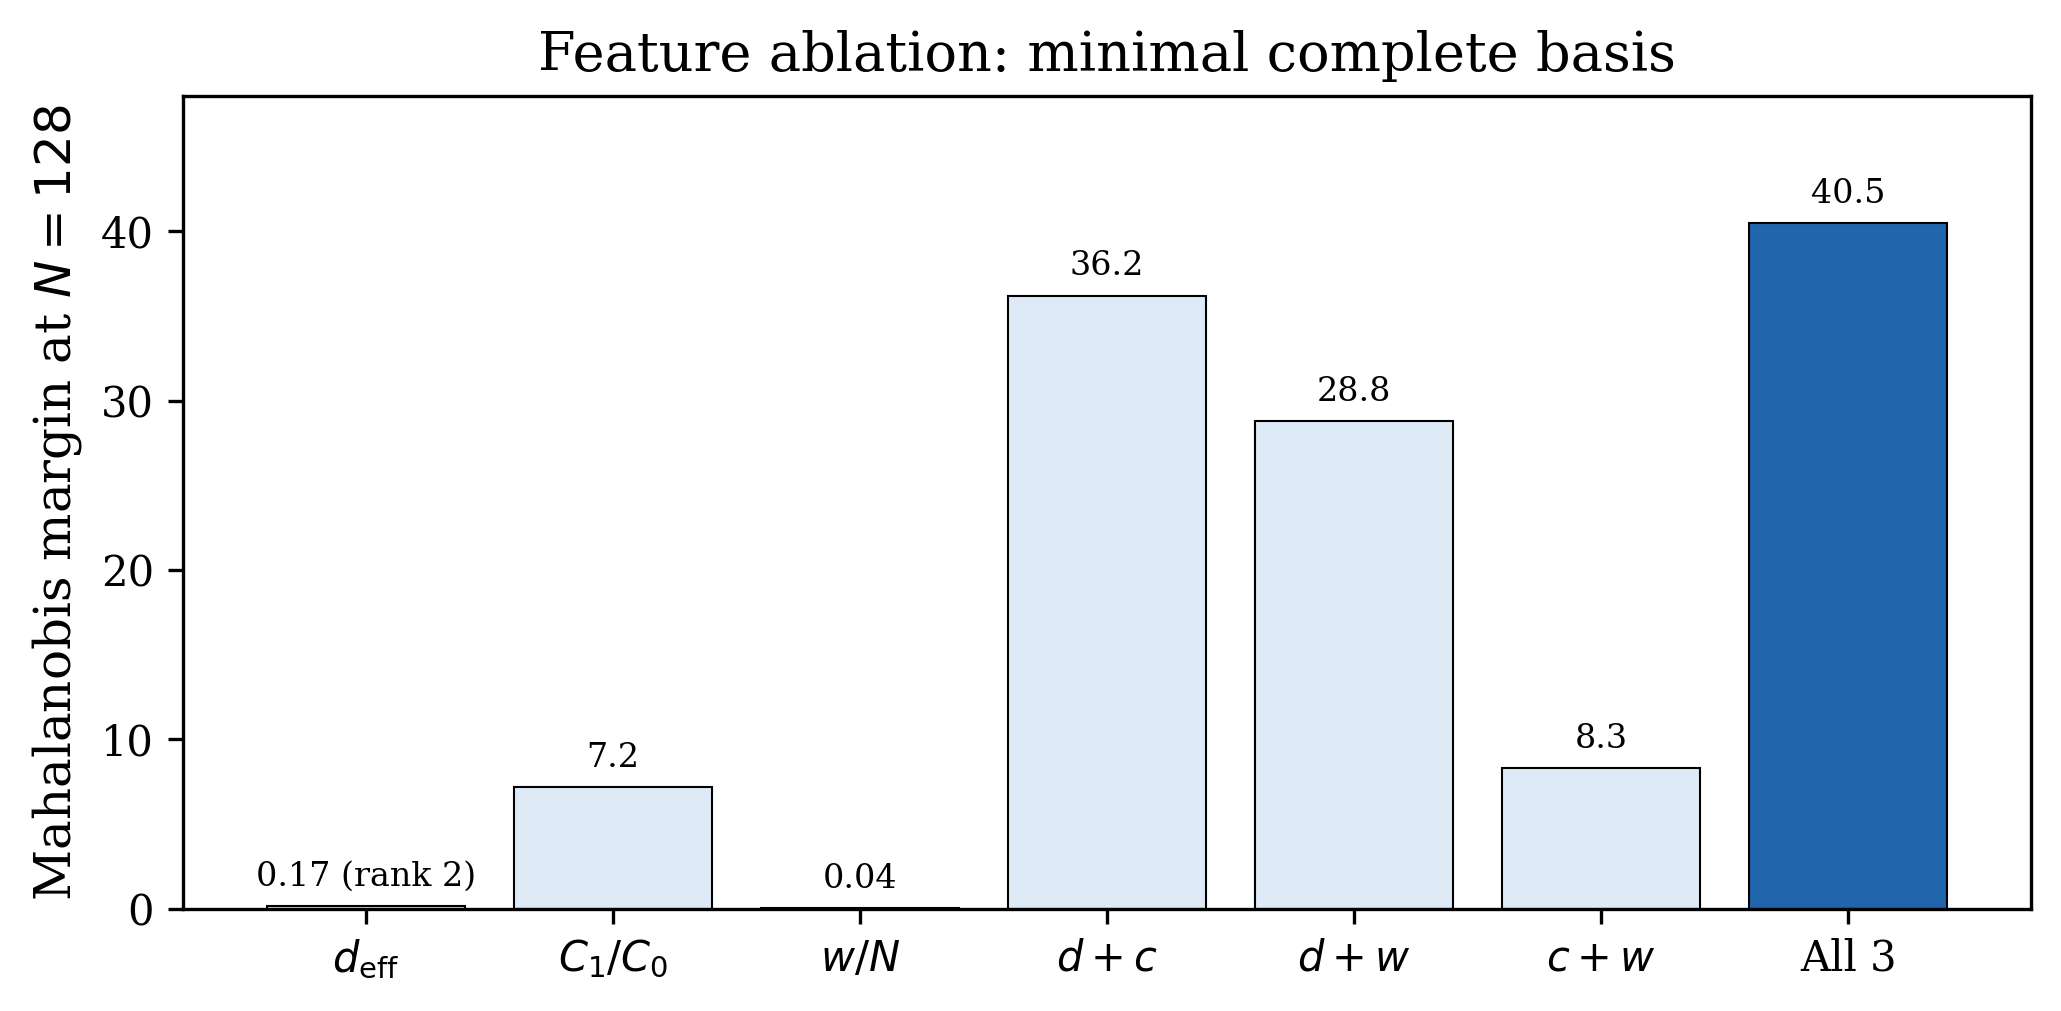
\includegraphics[width=0.65\textwidth]{figures/fig05_feature_ablation.pdf}
\caption{Feature ablation at $N=128$. The full triple achieves the largest
margin ($+40.5$). $\deff$ alone fails (rank~2); $w/N$ alone has negligible
margin.}
\label{fig:ablation}
\end{figure}

\item Finite $N\leq 1024$; the reference manifold asymptotics are fits, not
  proofs.
\item Curvature robustness is background-dependent, not uniform.
\item The 25-family library, while extensive, does not exhaust all conceivable
  poset structures.
\end{enumerate}

\subsection{Information-theoretic non-circularity test}
\label{sec:info-penalty}

A potential criticism of the two-layer architecture is circularity: the geometric
features used by $\SMD$ might implicitly encode the Lor4D identity they are
designed to detect. To address this, we replace the entire geometric penalty
with five purely information-theoretic quantities---spectral entropy deficit,
degree heterogeneity, layer concentration, edge-density extremity, and interval
diversity deficit---none of which reference any geometric target. Under the
resulting action $A_4 = -\beta\log H + \gamma\,I_{\mathrm{info}}$:

\begin{enumerate}
\item At moderate penalty strength ($\gamma=0.2$), $\Lor$ is
  rank~\#1 at all $N\geq 20$, selected purely by entropy efficiency.
\item At strong penalty ($\gamma\geq 0.5$), $\Lor$ drops to
  rank~\#3, consistently behind KR\_2layer and Lor5D---precisely the
  families penalised most by geometric penalties. The information-theoretic
  and geometric penalty classes thus encode orthogonal quality dimensions.
\item Ablation identifies interval diversity deficit as the sole critical
  discriminator among the five terms. In raw action scores, this term
  penalises KR\_2layer (80\% of total penalty) more heavily than $\Lor$
  (58\%), meaning its retention \emph{helps} $\Lor$ by selectively
  suppressing competitors.
\item A systematic weight scan (19 configurations, $N\in\{10,20,40\}$,
  $\gamma\in[0,2]$) confirms that no single weight vector allows $\Lor$ to
  be rank~\#1 across all $(N,\gamma)$. The optimal weight is $N$-dependent,
  reflecting the different scaling rates of $\log H$ and $I_{\mathrm{info}}$.
\end{enumerate}

\noindent
Neither penalty class alone selects $\Lor$ uniquely at large $N$ and all
$\gamma$: geometric penalties select dimension ($d=4$) but not family type;
information-theoretic penalties select family type (Lorentzian-like) but not
dimension. This \emph{complementarity theorem} provides independent evidence
that the two-layer screening architecture reflects two genuinely distinct
structural axes, not a circular geometric prior.

Moreover, combining both penalty types additively into a single action
($P_{\mathrm{geo}} + I_{\mathrm{info}}$) performs \emph{worse} than either
alone---degrading $\Lor$'s rank by up to 14 positions in 11 of 15 tested
conditions. The doubled penalty overwhelms the entropy term in favour of
structurally bland families. This negative result confirms that the two penalty
classes must be applied \emph{sequentially} (as distinct screening layers), not
\emph{additively} in a single objective.

The physical grounding of the dominant information-theoretic discriminator
(interval diversity deficit) can be verified independently: the normalised
interval-size entropy is strictly monotone decreasing in spacetime dimension~$d$
for Lorentzian sprinklings ($H = 0.82$, $0.66$, $0.45$, $0.28$ at $d = 2$--$5$;
$N = 40$), reflecting the Alexandrov interval volume power law
$V \propto \tau^d$.

\subsubsection{Sequential screening simulation}

The prohibition on additive combination raises an immediate question:
can the two penalty classes be applied \emph{sequentially} within a single
Boltzmann--action framework?
We tested a two-step protocol:
Step~1 ranks all 17~families by a soft geometric action~$A_2$ at penalty
strength~$\gamma_1$ and retains the top-$K$ candidates;
Step~2 re-ranks the $K$~survivors by a pure information action~$A_4$ at an
independently chosen~$\gamma_2$.
With $(\gamma_1,\gamma_2,K) = (0,\;0.5,\;3)$ at $N=10$ and $N=20$, and
$(0.5,\;2.0,\;5)$ at $N=40$, this protocol achieves $\Lor$ rank~\#1 at
\textbf{all three scales}---including $N=40$, where no single penalty mode
alone can reach~\#1.
Across a $4\gamma\times 4\gamma\times 3K = 144$~parameter grid,
27~conditions yield $\Lor$~\#1, of which 8~are strict improvements
(marked~$\star$) over every single-mode result.
These conditions cluster in the \emph{soft pre-filter / hard selector}
regime: $\gamma_1\leq 0.2$ (gentle geometric admission, retaining $\Lor$ in
the shortlist) paired with $\gamma_2\geq 0.5$ (strong information
selection).
This provides the first quantitative validation that the two-layer principle
operates \emph{within} the Boltzmann path-integral framework, not merely as
a post~hoc classification.

\subsubsection{Identity anchoring via \texorpdfstring{$\SMD$}{S\_MD}
  in the action}

A complementary test embeds $\SMD$ directly into the Boltzmann exponent:
$A = -\beta\log H + \gamma\,I_{\mathrm{info}} + \alpha\,\SMD$.
When $\gamma=0$ (no penalty at all), $A=-\log H + \alpha\,\SMD$ with
$\alpha\geq 1.0$ suffices to select $\Lor$~\#1 at all $N$.
Even under over-penalised conditions ($\gamma=2.0$, where $I_{\mathrm{info}}$
alone degrades $\Lor$ to~\#3), adding $\alpha\geq 0.5$ restores $\Lor$~\#1.
This ``identity anchor'' effect confirms that $\SMD$ captures irreducible
structural information about $\Lor$ that is independent of any penalty
mode's entropy--penalty trade-off.
Because $\SMD$ is defined relative to a $\Lor$ reference manifold, its role is
inherently second-layer (presupposing admissibility) rather than stand-alone;
the non-circular information-theoretic penalties remain the first-layer
complement.

\subsubsection{Curvature-adaptive reference prototype: \texorpdfstring{$\mu(N,\kappa)$}{mu(N,kappa)}}
\label{sec:mu-kappa-prototype}

To probe curved-background extension without altering the main pipeline,
we implemented a lightweight prototype that compares two reference manifolds
at fixed $N$: a flat reference $(\mu(N,0),\Sigma^{-1}(N,0))$ estimated from
Lor4D samples, and an adaptive reference $(\mu(N,\kappa),\Sigma^{-1}(N,\kappa))$
estimated from FLRW($\kappa$) samples.
Scores are evaluated with the same Mahalanobis form,
\begin{align}
S_{\mathrm{MD}}^{\mathrm{flat}}(x)
&=(x-\mu(N,0))^\top\Sigma^{-1}(N,0)(x-\mu(N,0)),\\
S_{\mathrm{MD}}^{\mathrm{adapt}}(x)
&=(x-\mu(N,\kappa))^\top\Sigma^{-1}(N,\kappa)(x-\mu(N,\kappa)).
\end{align}

For a medium grid ($N=256,512,1024$, $\kappa=1.0$; reference reps $=20$,
evaluation reps $=8$), the ranking pattern is consistent at all $N$:
under flat reference, Lor4D is rank~\#1 and FLRW is rank~\#2; under adaptive
reference, FLRW becomes rank~\#1 and Lor4D rank~\#2.
The manifold offset norm lies in
$\|\mu(N,\kappa)-\mu(N,0)\|_2\approx0.53\text{--}0.56$ and
increases mildly with $N$.

This does not replace the flat-reference core claim.
Rather, it establishes technical feasibility for a background-conditioned
reference family $\{\mu(N,\kappa)\}$ and supports the interpretation that
curvature response is best modelled as manifold drift around the flat identity
centre, not as failure of the layered architecture itself.

% ============================================================
\section{Conclusion}
\label{sec:conclusion}
% ============================================================

We have presented numerical evidence for a layered structural screening
architecture that uniquely selects 4D Lorentzian causal sets from a 25-family
poset library across $N=10$--$1024$.

The key results are:
\begin{enumerate}
\item \textbf{Two-layer architecture.}
  Linear admissibility ($\SBD$) plus quadratic identity ($\SMD$) form an
  orthogonal screening pair whose intersection is $\{\Lor\}$.
\item \textbf{Zero parameters.}
  The reference manifold $(\bm{\mu}(N),\Sigma(N))$ is entirely determined by
  $\Lor$ ensemble statistics.
\item \textbf{Turn-on boundary.}
  Identity recognition turns on sharply at $N_{\mathrm{id}}\approx 10$.
\item \textbf{Historical sedimentation.}
  The misidentification cost grows without bound
  ($\Veff\propto N^{-1.66}$, Fisher $\propto N$,
  gap $\to 1.93\times 10^8$ at $N=1024$).
\item \textbf{Background-dependent curvature robustness.}
  De~Sitter and weak-field Schwarzschild pass; FLRW $\kappa=1.0$ is
  boundary-sensitive. A prototype adaptive manifold $\mu(N,\kappa)$
  indicates systematic reference-centre drift (\S\ref{sec:mu-kappa-prototype}).
\item \textbf{Information-theoretic non-circularity.}
  Replacing geometric penalties entirely with information-theoretic measures
  still selects $\Lor$ at moderate $\gamma$, but fails at strong $\gamma$
  and large $N$---confirming that the two layers encode complementary, not
  redundant, structural information (\S\ref{sec:info-penalty}).
  A sequential protocol with independent penalty strengths achieves $\Lor$
  rank~\#1 at all tested $N$ including $N=40$ where no single mode suffices,
  quantitatively validating the layered architecture within the Boltzmann
  path-integral framework.
\end{enumerate}

The layered screening principle---that robust dimension selection requires
functionally distinct mechanisms at different algebraic orders---may point toward
a deeper structure in the causal set path integral, where the entropy catastrophe
is resolved not by a single action minimum but by a hierarchy of screening layers.

% ============================================================
% References
% ============================================================

\begin{thebibliography}{99}

\bibitem{BenincasaDowker2010}
D.~M.~T.~Benincasa and F.~Dowker,
\emph{Scalar Curvature of a Causal Set},
\emph{Phys.\ Rev.\ Lett.}\ \textbf{104}, 181301 (2010),
arXiv:1001.2725.

\bibitem{Bombelli1987}
L.~Bombelli, J.~Lee, D.~Meyer, and R.~D.~Sorkin,
\emph{Space-time as a causal set},
\emph{Phys.\ Rev.\ Lett.}\ \textbf{59}, 521 (1987).

\bibitem{Dhar1978}
D.~Dhar,
\emph{Entropy and phase transitions in partially ordered sets},
\emph{J.\ Math.\ Phys.}\ \textbf{19}, 1711 (1978).

\bibitem{KleitmanRothschild1975}
D.~J.~Kleitman and B.~L.~Rothschild,
\emph{Asymptotic enumeration of partial orders on a finite set},
\emph{Trans.\ Amer.\ Math.\ Soc.}\ \textbf{205}, 205 (1975).

\bibitem{LoomisCarlip2018}
S.~Loomis and S.~Carlip,
\emph{Suppression of non-manifold-like sets in the causal set path integral},
\emph{Class.\ Quantum Grav.}\ \textbf{35}, 024002 (2018),
arXiv:1709.00064.

\bibitem{MathurSinghSurya2020}
A.~Mathur, A.~Singh, and S.~Surya,
\emph{Entropy and the link action in the causal set path-sum},
\emph{Class.\ Quantum Grav.}\ \textbf{38}, 045017 (2021),
arXiv:2009.07623.

\bibitem{Meyer1988}
D.~A.~Meyer,
Ph.D.\ thesis, MIT (1988).

\bibitem{Myrheim1978}
J.~Myrheim,
\emph{Statistical Geometry},
CERN Tech. Rep.\ TH-2538 (1978).

\bibitem{Proemel2001}
H.~J.~Pr\"omel, A.~Steger, and A.~Taraz,
\emph{Phase transitions in the evolution of partial orders},
\emph{J.\ Combin.\ Theory Ser.\ A}\ \textbf{94}, 230 (2001).

\bibitem{Surya2019}
S.~Surya,
\emph{The causal set approach to quantum gravity},
\emph{Living Rev.\ Relativ.}\ \textbf{22}, 5 (2019),
arXiv:1903.11544.

\end{thebibliography}

\end{document}
